\chapter[Occupation Resolved Conductance of the Kondo Effect]{Occupation Resolved Conductance of the Kondo Effect}\label{cha:mixed_valence_conductance}
% Probably should be called: Occupation resolved conductance of the Kondo effect

\epigraph{Po bitvě je každý generál.}{Czech proverb}%~\cite{Strauss1998}}

\noindent To my knowledge, the following work in this chapter is the first time that conductance and charge transitions have been simultaneously measured to resolve the conductance enhancement due to the Kondo effect as a function of the occupation in an experiment. The conductance enhancement from Kondo is most pronounced when the quantum dot is strongly coupled ($\mathrm{\Gamma/k_BT}>>1$) to the source and drain leads. Previous measurements of the Kondo effect focus on the conductance enhancement between Coulomb peaks. However, when the coupling is strong, charge transitions broaden and become challenging to convert into an occupation. The following work falls between the tightly confined window of strong coupling to see the Kondo effect and weak coupling, where charge transitions are easily measured. 

\section{Introduction}
Previous measurements of the Kondo effect in quantum dots study the temperature dependence of conductance between Coulomb peaks. It is in this so-called Kondo regime that the full charge of the electron is in the dot, so there is a definite net spin, and the theory is well understood~\cite{costi_kondo_mv_eo_regime, kondo_unitary}. In this regime, the Kondo temperature (Eq.~\ref{eq:kondo_temp}) sets a new, many-body scale and is used to universally scale the conductance (Eq.~\ref{eq:kondo_conductance}). This one-parameter scaling of conductance in the Kondo regime is used as one of the demonstrations of the Kondo effect. When the coupling between the quantum dot and source and drain leads is reduced, the Kondo temperature drops below the system temperature, and the conductance enhancement is not seen between Coulomb peaks. Only a handful of experiments have studied conductance with less strong coupling~\cite{goldhaber_mv}. Such studies observed the parameter $\mathrm{s}$ from Eq.~\ref{eq:kondo_conductance} and found that in the Kondo regime (the full charge of the electron is in the dot), $\mathrm{s}$ was constant and equal to $0.20$. However, as the shoulder of a Coulomb peak was approached ($\tilde{\epsilon}_0>-0.5$), $\mathrm{s}$ varied rapidly. Qualitatively, this regime is entered when the dot energy $\epsilon_0$ approaches the Fermi energy of the leads, and only a fraction of the electron charge is in the dot. 


Our aim was to measure the Kondo effect with a coupling strength such that the conductance between Coulomb peaks was zero. This regime, characterised by a relatively small $\Gamma$, results in a small Kondo temperature between Coulomb peaks, and no conductance enhancement would be measured. However, the Kondo temperature will increase as the dot energy approaches the Fermi energy of the leads (moves towards the shoulder of a Coulomb peak). Hence, for relatively small coupling strengths, the Kondo effect can still be seen as a very small conductance enhancement on the odd occupied side of a Coulomb peak. As the conductance enhancement in this regime is very small, it is insufficient to investigate the Kondo effect with a conductance measurement only, for two reasons. Firstly, entropy shifts the occupation of the quantum dot with temperature. This effect has been taken advantage of in a recently developed entropy measurement technique~\cite{hartman, child_strong, child_meas}. This shift in occupation can be ignored when the coupling is strong, and conductance enhancement between Coulomb peaks is large. Secondly, charge motion in the dopant layer can shift the conductance left or right with respect to the gate voltage in a scan. The shifting from charge motion renders it impossible to offset the effects of entropy by retroactively shifting conductance. 

For these two reasons, it is necessary to simultaneously measure a second `reference' signal alongside the conductance. This reference signal can then be used to offset the above effects and allow for comparison of the conductance across multiple temperatures. We measure the charge in the quantum dot simultaneously with conductance. Assuming a linear relation between the measured change in charge and the real occupation of the quantum dot, the charge transition is converted into an occupation. The occupation is then used to plot the conductance as a function of occupation. A shifting of the conductance maximum to a higher occupation is a signature of the Kondo effect. 
As the universal scaling of conductance does not hold in this regime, a comparison to theory calculations (described in an upcoming section) is required to verify Kondo enhancement. 





\section{Occupation Resolved Conductance Method}
The conductance and charge of the quantum dot are simultaneously measured to investigate the small enhancement of conductance due to the Kondo effect with relatively small coupling. On the hardware side, a simultaneous measurement of the charge and conductance is trivial as two different current amplifiers are simply connected to the device. 
The first current amplifier measures the conductance through the quantum dot and the other, current through the charge sensor. Each current amplifier is connected to two analog-to-digital converters (ADCs), which sample data points simultaneously. 
Conductance is measured using a pseudo-lockin technique. Here a DAC channel voltage biases the current amplifier using a \qty{\pm1}{\micro V} square wave. The underlying signal is recovered in analysis by multiplying with a sine wave of equal frequency and averaging all the points per square wave cycle. This technique mitigates the effects of bias drift in the current amplifier so that a reliable \qty{1}{\micro V} source-drain bias is applied across the dot. 
A \qty{100}{\micro V} DC bias is applied across the charge sensor. Large source-drain bias across the charge sensor can de-phase the Kondo singlet~\cite{kondo_controlled_dephasing}, however, a range of 50-\qty{250}{\micro V} source-drain biases was tested with no significant effect.

It is much trickier to tune the quantum dot into a regime where both the conductance and charge transition can be compared to theory. When weakly coupled ($\mathrm{\Gamma/k_BT}<<1$), the charge transitions have a sharp drop in current and can be fit analytically using Eq.~\ref{eq:cs_lineshape}. However, a weakly coupled Coulomb peaks amplitude drops with the strength of coupling~\cite{Kouwenhoven_1997_electron_transport} as,


\begin{equation}\label{eq:cond_amp}
 \mathrm{G_0} \propto
 \frac{\Gamma_\mathrm{L}\cdot\Gamma_\mathrm{R}}{\Gamma_\mathrm{L}+\Gamma_\mathrm{R}}
\end{equation}


\noindent where $\mathrm{G_0}$ is the conductance maximum. This decrease in conductance amplitude means that the conductance signal can be lost within the background noise. Additionally, as the Kondo temperature decreases with reduced coupling, the conductance enhancement due to Kondo can become immeasurable.


Alternatively, in a strongly coupled regime ($\mathrm{\Gamma/k_BT}>>1$), Coulomb peaks are usually easier to measure. Here the line shape for a Coulomb peak is given by the Breit-Wigner formula~\cite{Breit1936}. The conductance is maximum when the dot energy is in line with the Fermi energy of the leads and depends on the coupling as 

\begin{equation}\label{eq:cond_amp_strong}
 \mathrm{G_0} \propto
 \frac{\Gamma_\mathrm{L}\cdot\Gamma_\mathrm{R}}{\left(\Gamma_\mathrm{L}+\Gamma_\mathrm{R}\right)^2}
\end{equation}

\noindent In both weakly and strongly coupled regimes, it is evident that the conductance reaches a maximum when the tunnel barriers are symmetric ($\Gamma_\mathrm{L}=\Gamma_\mathrm{R}$). Strong coupling also has the added benefit of an increase in Kondo temperature, leading to greater enhanced conductance. 
However, as Coulomb peaks become easier to measure, charge transitions become very broadened and difficult to measure (Fig.~\ref{fig:ch1/virtual_gate_example}). When strongly coupled, large sweeps in gate voltage are required to cover a range where the quantum dot is fully unoccupied to occupied. This can result in the charge sensor being pushed into a non-linear regime due to the cross-capacitive coupling from the sweep gate.
A non-linear relationship between the current through the charge sensor and the addition of charge into the quantum dot makes extraction of dot occupation from the charge transition unreliable. Hence, a virtual gate shown in Fig.~\ref{fig:ch1/virtual_gate_example}, that keeps the current through the charge sensor constant is required. The exact ratio of gates used to form a virtual gate can drastically change the underlying shape of the charge transition, which will be discussed in an upcoming section. 


\subsection{Numerical Renormalisation Group (NRG)}
The dot is carefully tuned to a coupling regime where the conductance enhancement due to Kondo is expected, and charge transitions are reliably measured. As previous tests of the Kondo effect are not possible in this regime, a comparison to Numerical Renormalisation Group (NRG) calculations~\cite{nrg} is required. Our theory collaborators (Yigal Meir, Yaakov Kleeorin, and Andrew Mitchell) provide these calculations. 
Two 2D datasets corresponding to conductance and occupation are received.The columns are energy scaled by $\Gamma$ (energy/$\Gamma$), so the x-axis is unitless. The rows in the 2D datasets correspond to a different $\mathrm{\Gamma/k_BT}$ value. We confirmed with Yaakov that the lineshape does not change if both $\mathrm{T}$ and $\mathrm{\Gamma}$ increase together. The lineshape represents the ratio $\mathrm{\Gamma/k_BT}$, not $\mathrm{\Gamma}$ or $\mathrm{T}$ individually.

To compare NRG to data, $\mathrm{\Gamma/k_BT}$ should be reliably determined so the correct row from NRG is used. Then, the correct scaling is applied to convert the NRG into measurement units. Conductance and charge transitions have similar scaling parameters. Amplitude, x-offset and lever arm which scales the NRG x-axis in units of mV. The occupation NRG has extra parameters: a y-offset, which comes from the current through the charge sensor; a linear term, which comes from the cross-capacitance between the sweep gate and charge sensor; and an occupation-dependent linear term. 
This occupation-dependent linear term reflects a change in the cross-capacitance as an electron enters the quantum dot. In Fig.~\ref{fig:ch3/cond_occ_QPC_vs_ct}, the charge transition slopes are different between the unoccupied (left) and occupied (right) sides. We argue that the additional charge of an electron in the quantum dot can give rise to such a change in cross-capacitance. Many of these parameters have low cross-correlation when fitting data to NRG, meaning the global minimum of the minimiser is reliably reached. However, this is not true for the parameters $\mathrm{\Gamma/k_BT}$ and lever arm. Changes to $\mathrm{\Gamma/k_BT}$ can be offset by a change in lever arm, and fitting a single trace allowing both parameters ($\mathrm{\Gamma/k_BT}$ and lever arm) to vary freely is unreliable. 


\subsection{Conductance Global Fit to NRG}
In the temperature broadened regime ($\mathrm{\Gamma/k_BT} < 1$), $\mathrm{\Gamma/k_BT}$ and lever arm are decoupled as the broadening of the conductance or charge transition is from temperature only. To access the temperature broadened regime from the gamma broadened regime ($\mathrm{\Gamma/k_BT} > 1$), the temperature of the fridge is increased until $\mathrm{\Gamma/k_BT} \lesssim 1$. Figure~\ref{fig:ch3/cond_ct_gf} shows that data is taken at multiple temperature setpoints across this range so that $\mathrm{\Gamma/k_BT}$ and lever arm can be reliably determined. Conductance and charge transitions are simultaneously measured at each temperature. However, only the conductance data is used to determine $\mathrm{\Gamma/k_BT}$ and lever arm, as it is generally cleaner. A global fit to the conductance data, including each temperature setpoint, is used in Fig.~\ref{fig:ch3/cond_ct_gf}\textbf{a}. Here $\mathrm{\Gamma}$ and lever arm are allowed to vary, but held fixed between temperatures, and $\mathrm{T}$ is held fixed to the calculated electron temperatures from Fig.~\ref{fig:ch1/electron_temp}. The other parameters (amplitude and x-offset) used to fit the NRG to conductance data are allowed to vary freely.
The fitting range is the full width at $90\%$ the maximum conductance. This removes any bias of picking a `good' fitting range. 

\subsection{Charge Transition Fit to NRG}
Each charge transition is fit separately to NRG, where $\mathrm{\Gamma/k_BT}$ and lever arm determined from the conductance global fit, are held fixed. All other parameters (amplitude, x-offset, y-offset, linear and occupation-dependent linear) are allowed to vary freely (Fig.~\ref{fig:ch3/cond_ct_gf}\textbf{b}). The fitting range of the charge transitions is maximised up to, but excluding charge jumps.


\begin{figure}[H]
 \begin{center}
%% includegraphics: comment the following if not using the graphicx package
 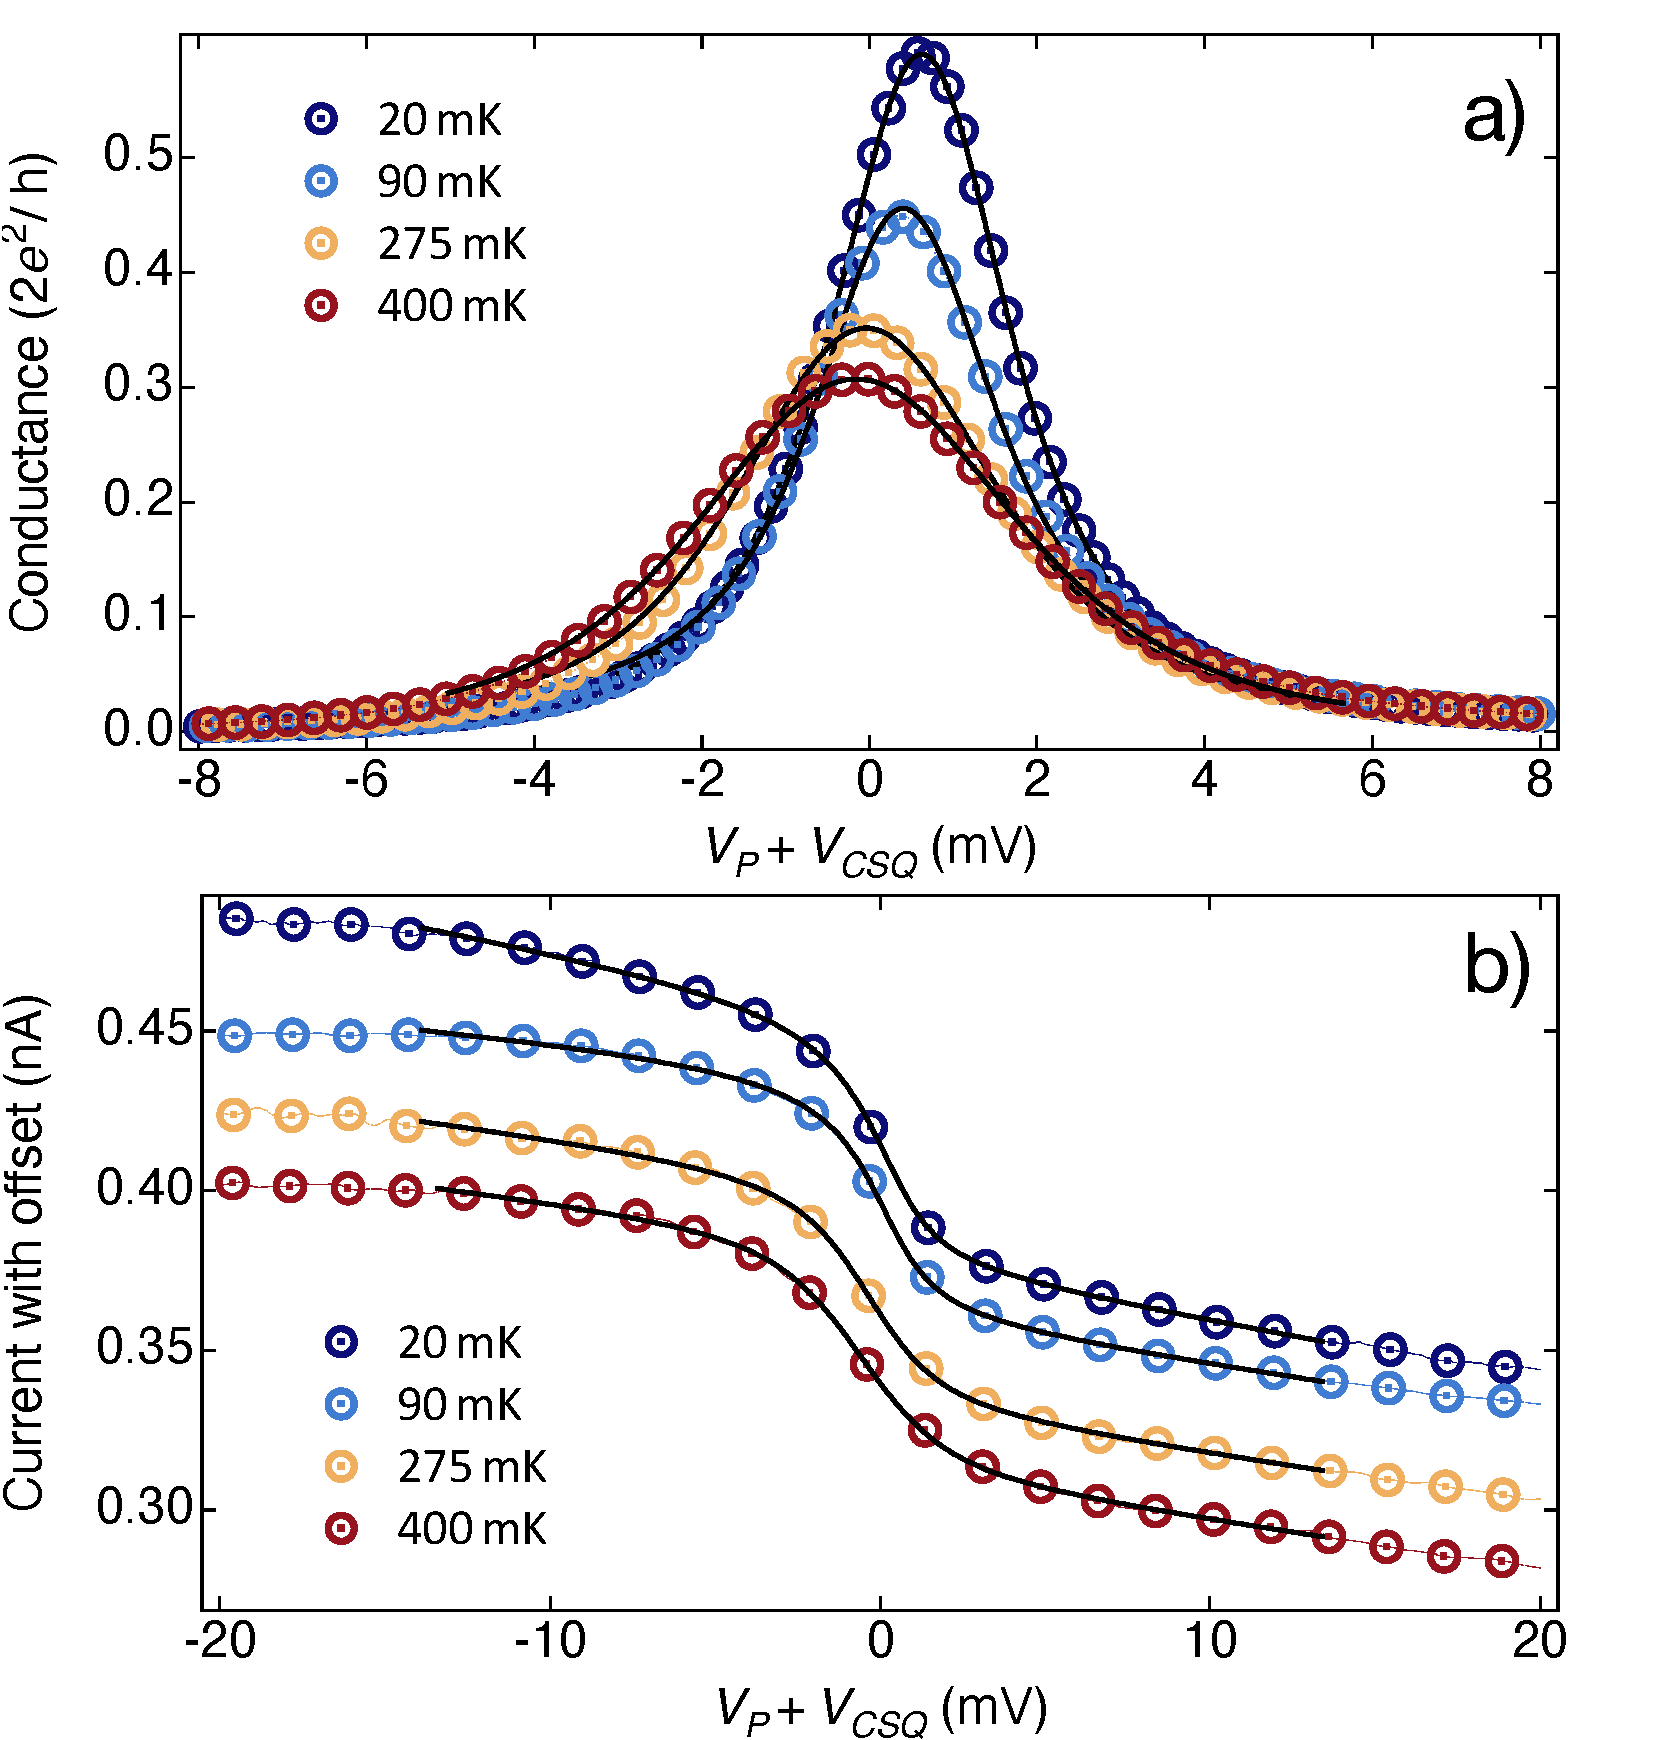
\includegraphics[width=0.85\textwidth]{figures/ch3/figure13.pdf}
 \caption[Fit Conductance and Charge Transition to NRG]{\label{fig:ch3/cond_ct_gf} 
 % For some options that work with pdf\LaTeX, please see this discussion:
 % \url{http://tex.stackexchange.com/questions/11839}. 
 (\textbf{a}) Conductance as a single electron enters a strongly coupled ($\mathrm{\Gamma/k_BT > 1}$) quantum dot at four different temperatures. The x-location of the conductance maximum has not been shifted and is the original x-location of the measured data. The fits (in grey) are from a global fit to NRG, where the $\Gamma$ and lever arm parameters are held fixed across all four temperatures. (\textbf{b}) Charge transitions are measured simultaneously with the conductance. Each charge transition is separately fit to NRG, where the $\Gamma$ and lever arm parameters are held fixed to the values determined from the global fit to conductance.}
 \end{center}
\end{figure}



% \newpage

\subsection{Determining Occupation}

\begin{figure}[!hbt]
 \begin{center}
 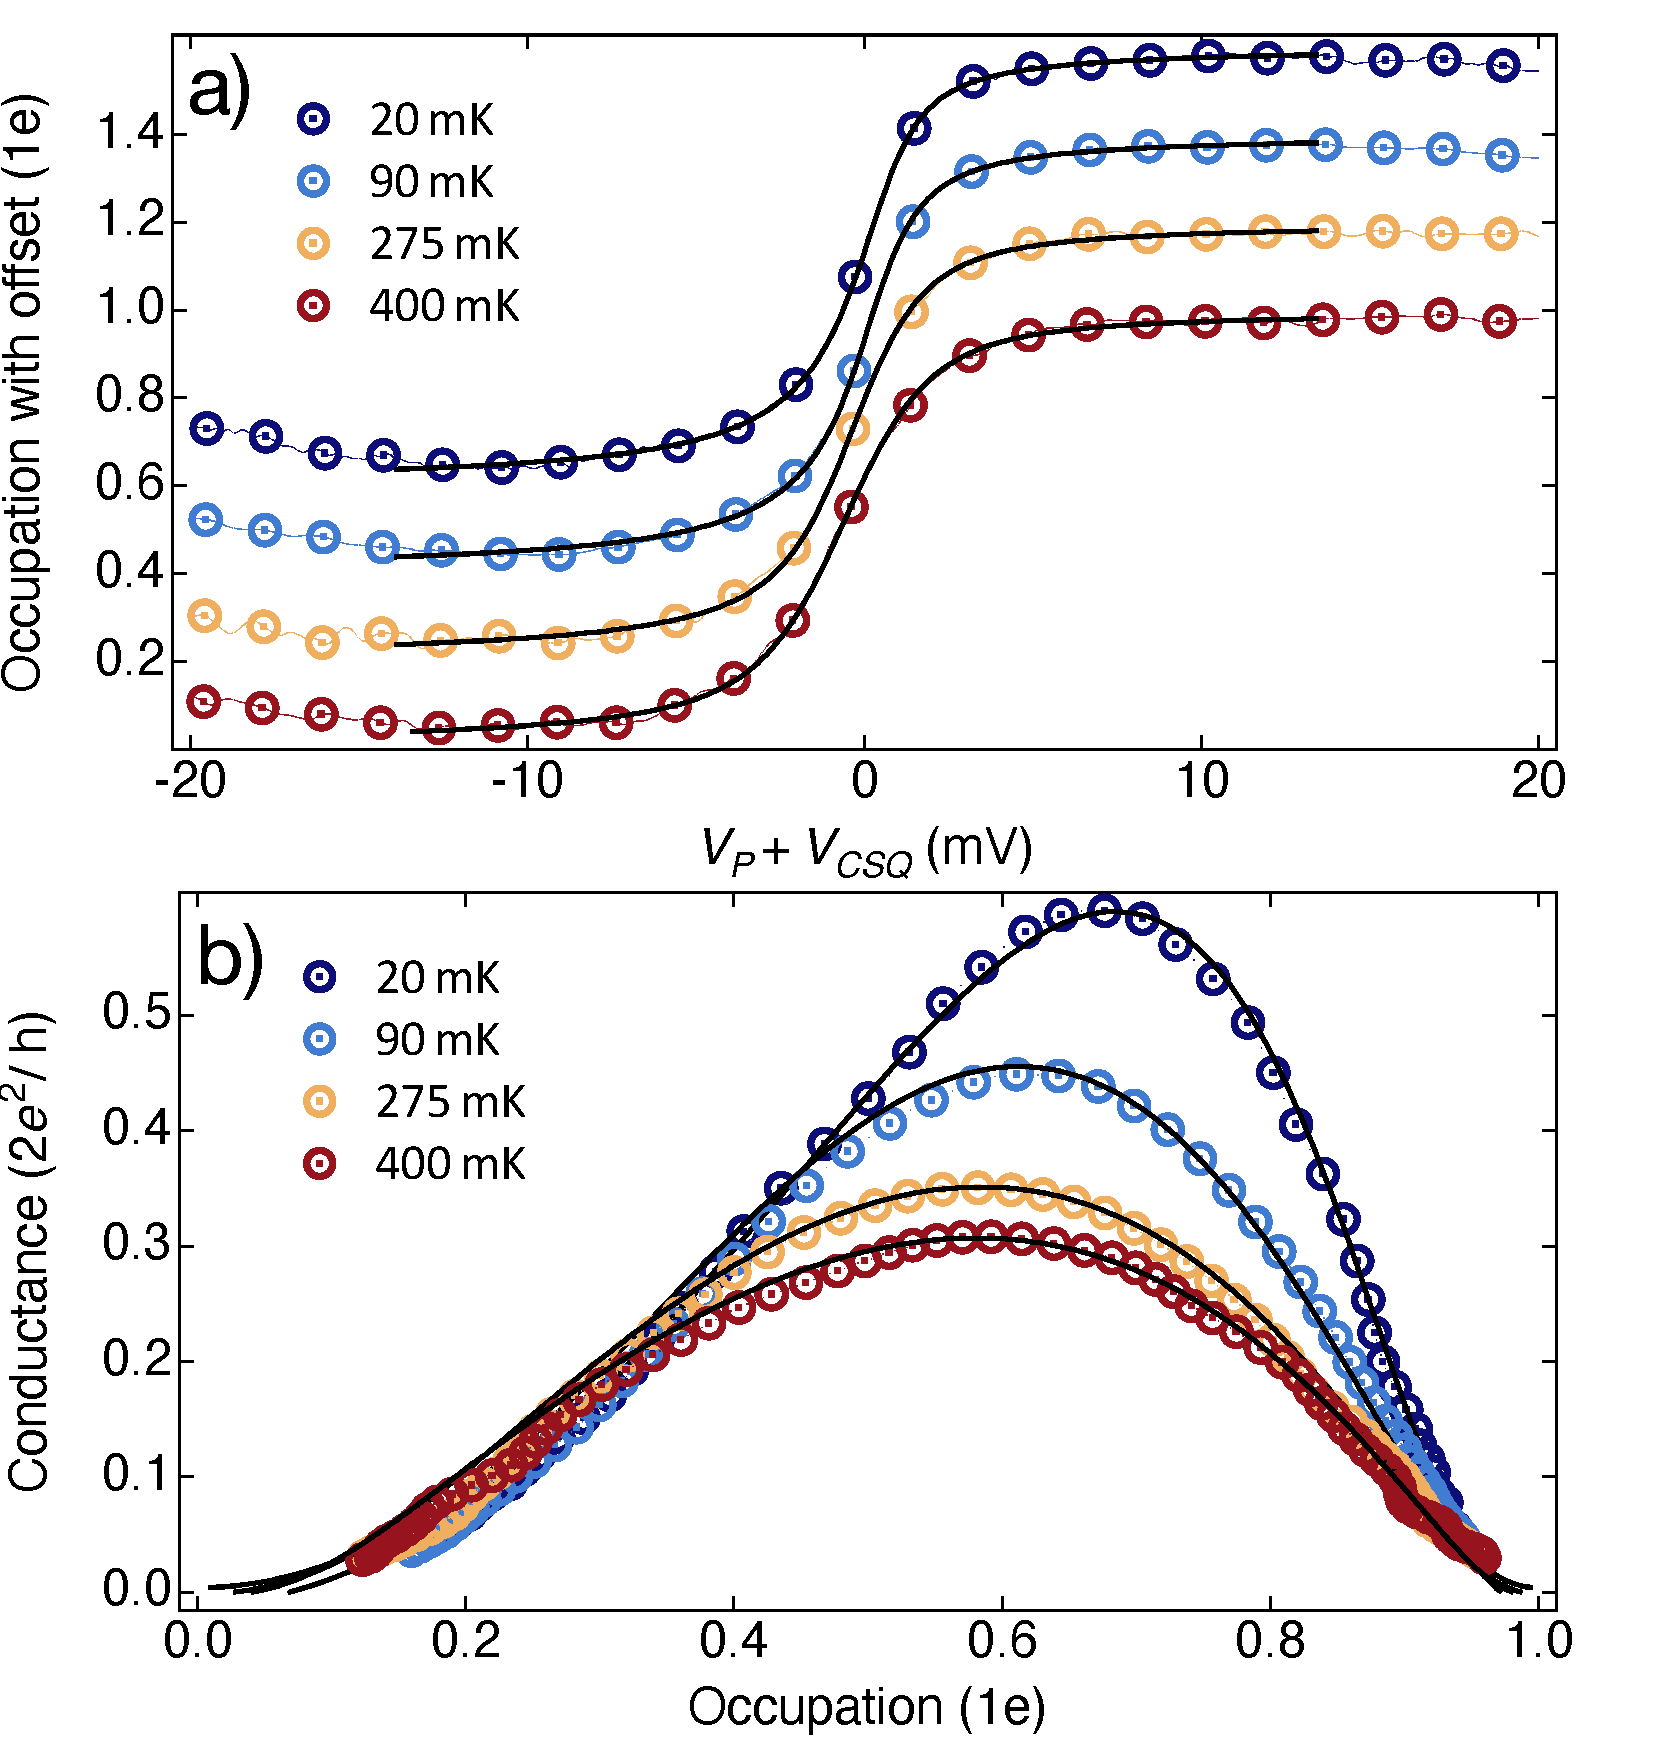
\includegraphics[width=0.85\textwidth]{figures/ch3/figure14.pdf}
 \caption[Conductance versus Occupation : Varying Temperature]{\label{fig:ch3/cond_vs_occ_gf} 
 % For some options that work with pdf\LaTeX, please see this discussion:
 % \url{http://tex.stackexchange.com/questions/11839}. 
 (\textbf{a}) Charge transitions are converted to occupation by removing the relevant fit parameters. These are amplitude, current offset, cross-capacitance of virtual gate, and occupation-dependent cross-capacitance. (\textbf{b}) Conductance versus occupation is used to show the enhanced conductance due to Kondo. As temperature decreases, the conductance maximum occurs at greater occupation. The NRG (grey) conductance versus occupation corresponding to the determined $\mathrm{\Gamma/k_BT}$ is plotted on top of the data, where good agreement is found at each temperature.}
 \end{center}
\end{figure}


The charge transition cannot be used as a reference to compare with conductance due to changing amplitude and linear terms with changes in dot settings. However, charge transitions can be converted into an occupation, allowing for the comparison of conductance enhancement between dot settings. The fit parameters from the NRG fit to the charge transitions are used to remove relevant terms. The current offset (y-offset) and linear term are removed trivially. The occupation-dependent linear term is removed by multiplying this linear term with the correct NRG occupation row corresponding to $\mathrm{\Gamma/k_BT}$. Lastly, the charge transition is re-scaled by the amplitude. NRG only has to be shifted by the x-offset and scaled by the lever arm to make a comparison with data (Fig.~\ref{fig:ch3/cond_vs_occ_gf}\textbf{a}).


\subsection{Conductance versus Occupation}

Plotting conductance versus occupation overcomes the issue of conductance shifting due to entropy or charge motion. Figure~\ref{fig:ch3/cond_vs_occ_gf}\textbf{b} shows the conductance data plotted against the determined occupation. Conductance enhancement due to Kondo can be seen from a shift of the conductance maximum to occupation greater than 0.5 (N $>0.5$). This shift in the conductance maximum indicates that even as the dot energy of the quantum dot falls below the energy level of the leads, there is enhanced conductance due to the formation of a Kondo singlet. As the temperature is lowered in Figure~\ref{fig:ch3/cond_vs_occ_gf}\textbf{b}, the conductance maximum shifts to higher occupation. This is because the system temperature falls below the Kondo temperature, and the Kondo singlet remains formed. As the conductance and occupation data are fit to different ranges, it is essential to ensure that the conductance and occupation data points plotted against each other correspond to the same gate voltage. The NRG conductance versus occupation in Fig.~\ref{fig:ch3/cond_vs_occ_gf}\textbf{b}, is the unscaled NRG provided by the theorists corresponding to $\mathrm{\Gamma/k_BT}$. There is good agreement between the data and NRG at each temperature. 



\section{Kondo Effect with Varying Coupling Strength}


\begin{figure}[!hbt]
 \begin{center}
%% includegraphics: comment the following if not using the graphicx package
 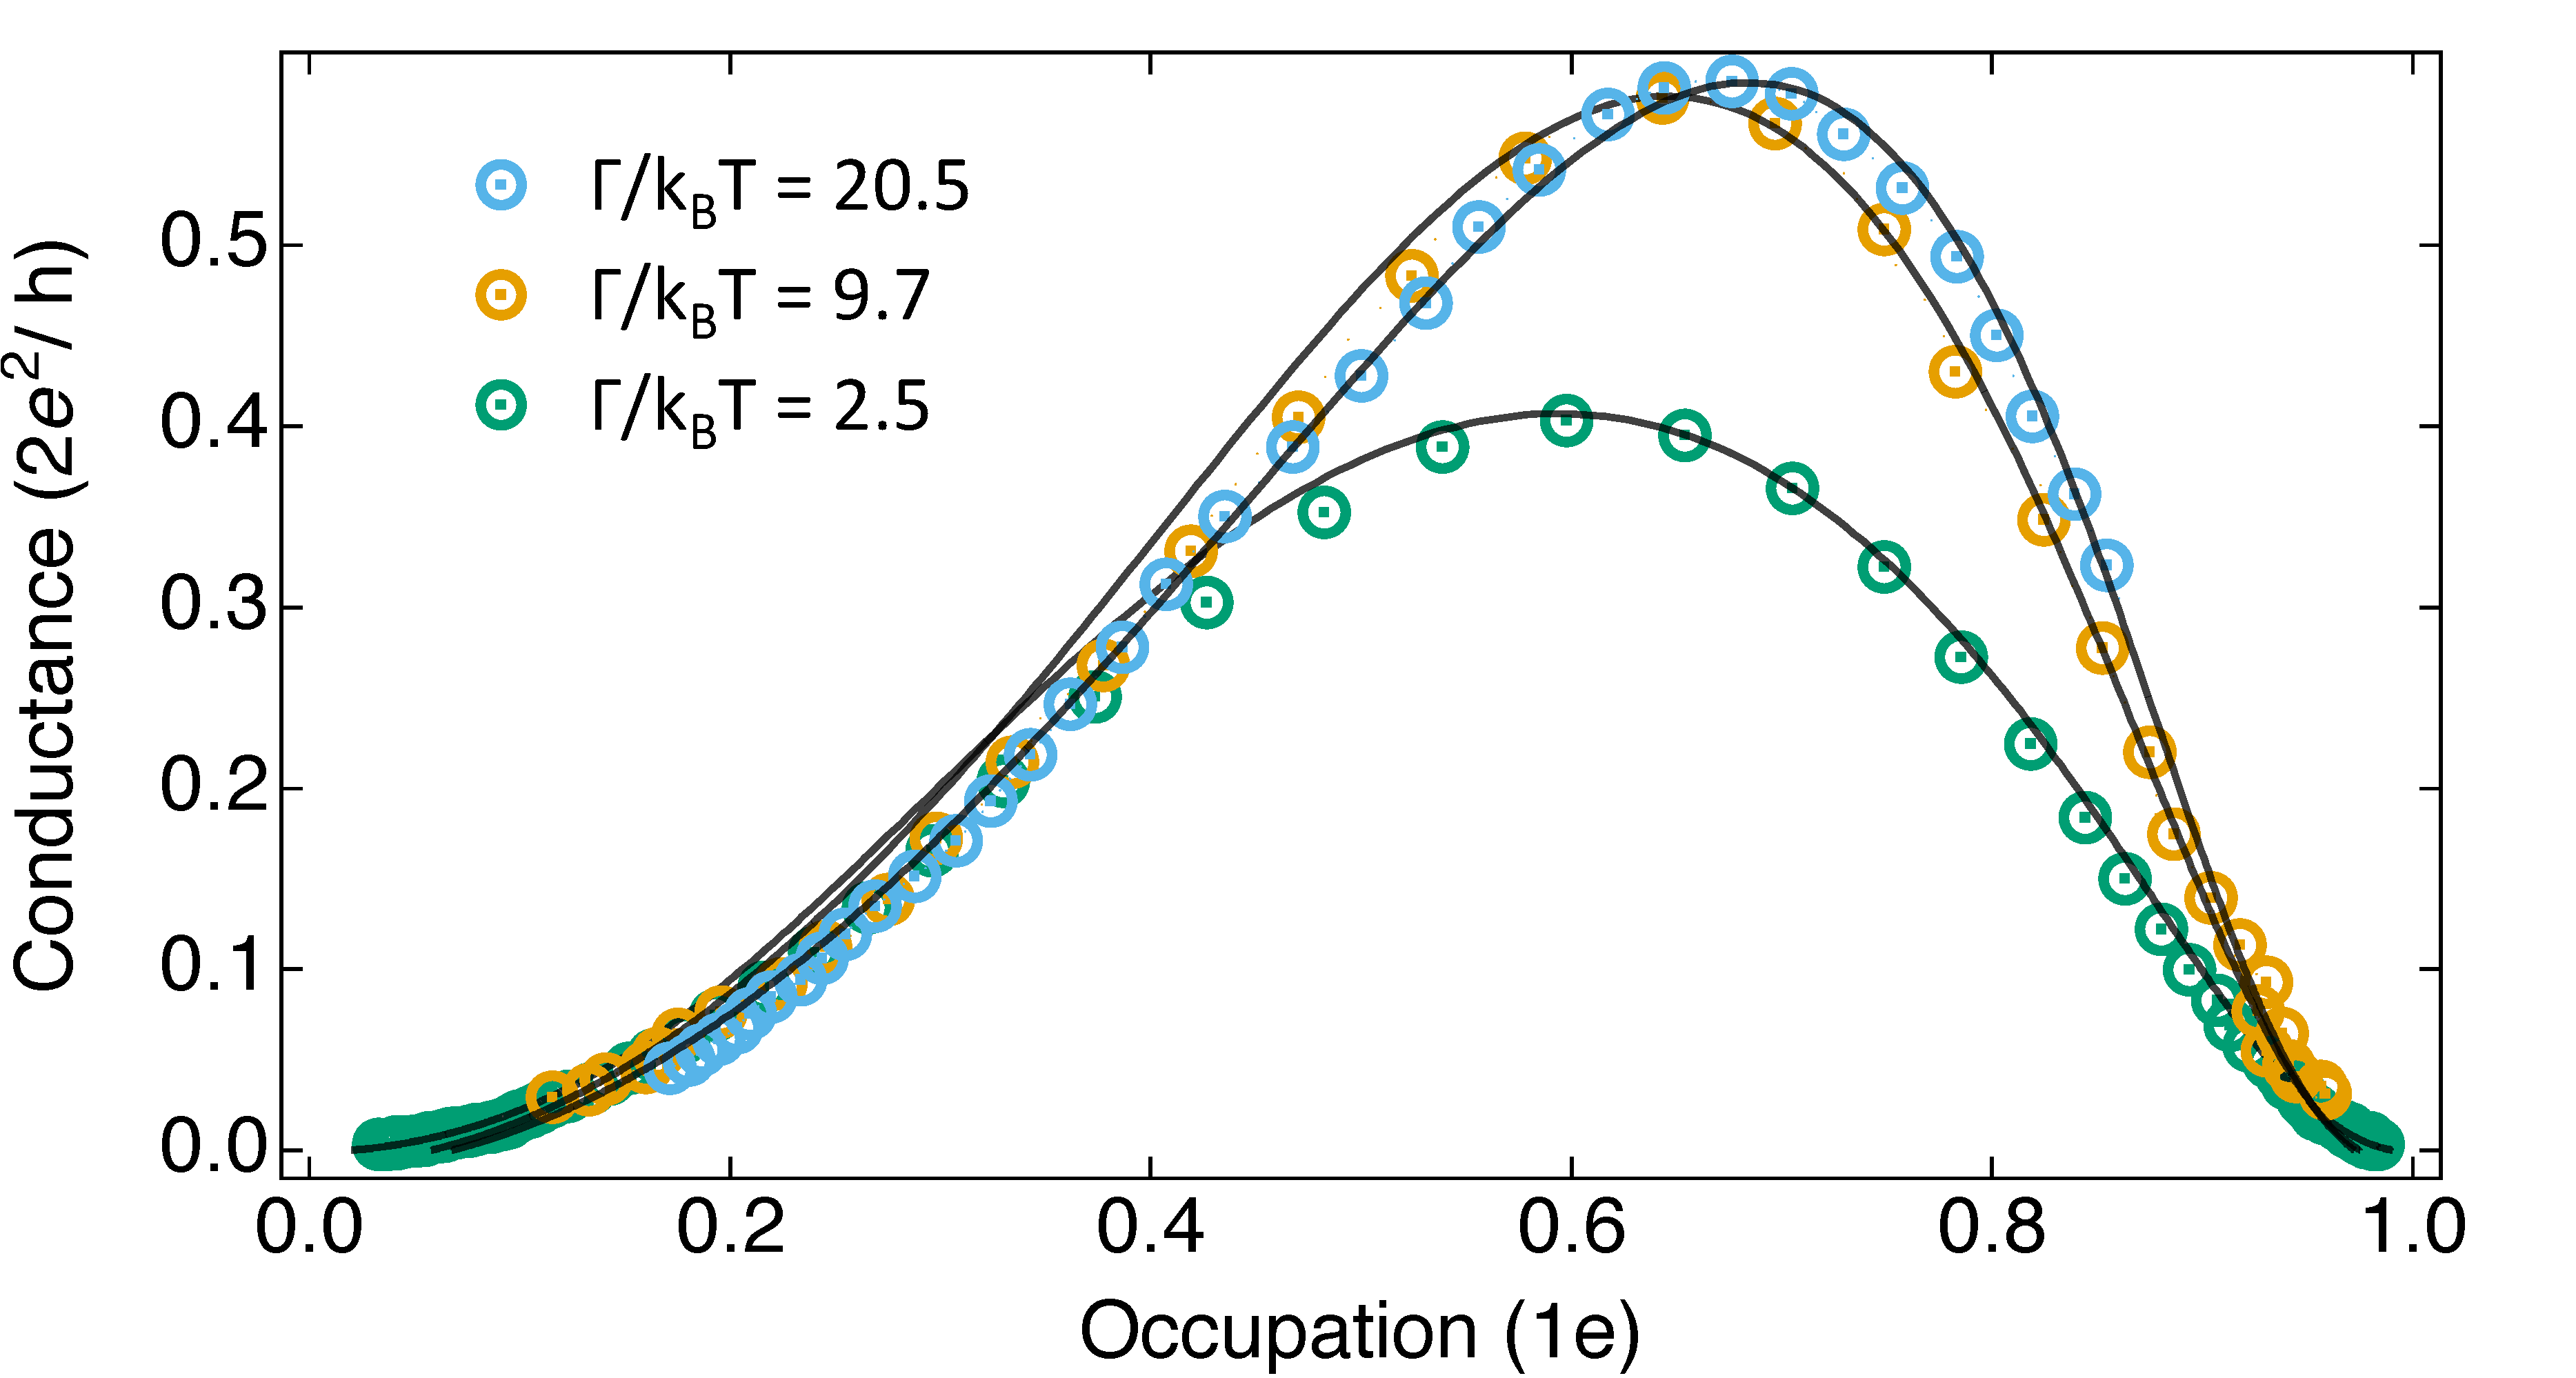
\includegraphics[width=0.85\textwidth]{figures/ch3/figure15.pdf}
 \caption[Conductance versus Occupation : Varying Coupling Strength]{\label{fig:ch3/cond_occ_couplingstrength} 
 % For some options that work with pdf\LaTeX, please see this discussion:
 % \url{http://tex.stackexchange.com/questions/11839}. 
 Conductance versus occupation in a weak (green) and strong (blue) coupling regime. Each trace is taken at \qty{20}{mK}. The coupling strength $\mathrm{\Gamma/k_BT}$ was determined from a global fit to multiple temperatures. The NRG (grey) conductance versus occupation corresponding to the determined $\mathrm{\Gamma/k_BT}$ is plotted on top of the data. Good agreement is found at each coupling strength.}
 \end{center}
\end{figure}


In Fig.~\ref{fig:ch3/cond_vs_occ_gf}\textbf{b}, the Kondo enhancement dependence on the system's temperature was confirmed. At high temperatures $\mathrm{T>T_K}$, there is no Kondo singlet, and so the conductance maximum is near $\mathrm{N} = 0.5$. But at low temperatures $\mathrm{T<T_K}$, a Kondo singlet is formed, and the conductance maximum shifts to higher occupation $\mathrm{N} > 0.5$. This displays the dependence of the Kondo temperature on the dot energy. The Kondo temperature rises as the dot energy gets close to the leads. However, the Kondo temperature also depends on the coupling strength between the quantum dot and leads Eq.~\ref{eq:kondo_temp}. As strongly coupled quantum dots have larger Kondo temperatures, the conductance maximum is expected to occur at higher occupation than in weakly coupled quantum dots. 



Figure~\ref{fig:ch3/cond_occ_couplingstrength} shows \qty{20}{mK} traces of conductance versus occupation at three different coupling strengths. $\mathrm{\Gamma/k_BT}$ is determined using the fitting routine described above to plot the corresponding NRG alongside the data. Expectedly, the more strongly coupled data shows a greater shift in the conductance maximum to higher occupation. Good agreement with NRG is observed at each coupling.






% \afterpage{\clearpage}
% \afterpage{}
% \FloatBarrier
\section{Kondo Effect with Varying Charge Sensor Current}

This new method of plotting conductance versus occupation not only requires a reliable determination of $\mathrm{\Gamma/k_BT}$ and lever arm from conductance data, but also clean charge transitions that can be converted into an occupation. The shape of the charge transition can vary depending on the choice of virtual gate and the charge sensor QPC setpoint. In the next section, different current setpoints of the charge sensor QPC are measured and the resulting conductance versus occupation is tested for agreement with NRG.


% \afterpage{\clearpage}
\subsection{Varying Charge Transition}


\begin{figure}[!bht]
 \begin{center}
%% includegraphics: comment the following if not using the graphicx package
 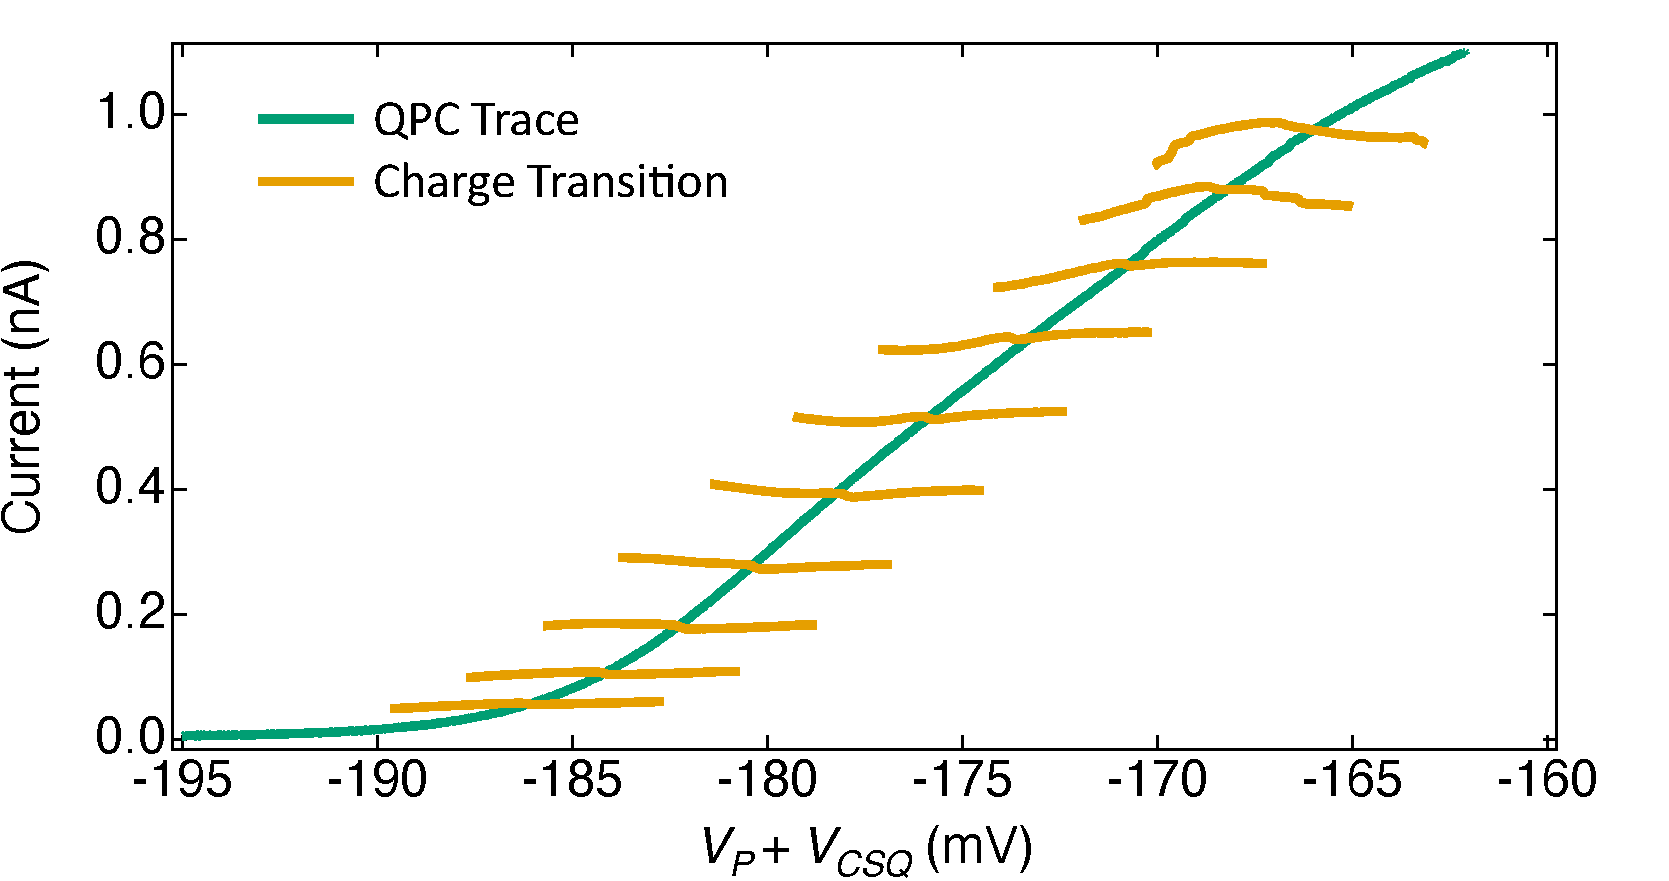
\includegraphics[width=0.85\textwidth]{figures/ch3/figure16.pdf}
 \caption[Varying Charge Sensor Current Setpoint]{\label{fig:ch3/cond_occ_ct_set-points} 
 % For some options that work with pdf\LaTeX, please see this discussion:
 % \url{http://tex.stackexchange.com/questions/11839}. 
 Current through the charge sensor (green) from pinch-off to the start of the first conductance plateau. Corresponding charge transition (yellow) at each current setpoint through the charge sensor. Note the x-axis is different between the underlying charge sensor trace and charge transitions. The charge transitions x-axis has been scaled the same amount for clarity. The charge transitions vary dramatically as the current through the charge sensor is changed. The left and right slopes curve upwards, downwards, in the same direction, or opposite each other.}
 \end{center}
\end{figure}
% \FloatBarrier


Figure~\ref{fig:ch3/cond_occ_ct_set-points} shows a charge sensor trace (green) and the resulting charge transition (yellow) at a range of current setpoints through the charge sensor. The current (y-axis) has not been scaled differently between the charge sensor trace and charge transitions. However, the sweep gate (x-axis) of the charge sensor and charge transitions are different. The charge transition sweep gate axis has been scaled for clarity in this plot. 



The shape of the charge transition varies significantly as the current setpoint through the charge sensor changes. Typically, the charge sensor is set to its steepest slope where the derivative is the largest. Here, the charge sensor is most sensitive as small changes in the potential result in large changes in the current. The resulting amplitude of the charge transition is greatest at the steepest slope. However, charge transitions can be measured at any current setpoint through the charge sensor. As long as the change in current through the charge sensor is linear with respect to the change in voltage. This can be achieved with a virtual gate, which keeps the current through the charge sensor constant. 



Yet, at each charge sensor current setpoint, the charge transition slopes vary differently on the unoccupied and occupied sides. Comparing the slopes on the unoccupied (left) side, at low currents, they point downwards, then point upwards with increasing current, and then point downwards again at the highest current setpoint. It is important to show that the conduction versus occupation agrees with NRG, irrespective of the current setpoint through the charge sensor. Otherwise, it may be possible to `pick' a current setpoint through the charges sensor that either shows or does not show agreement with NRG. This would render the method unreliable. 




\subsection{Conductance versus Occupation}



\begin{figure}[!hbt]
 \begin{center}
%% includegraphics: comment the following if not using the graphicx package
 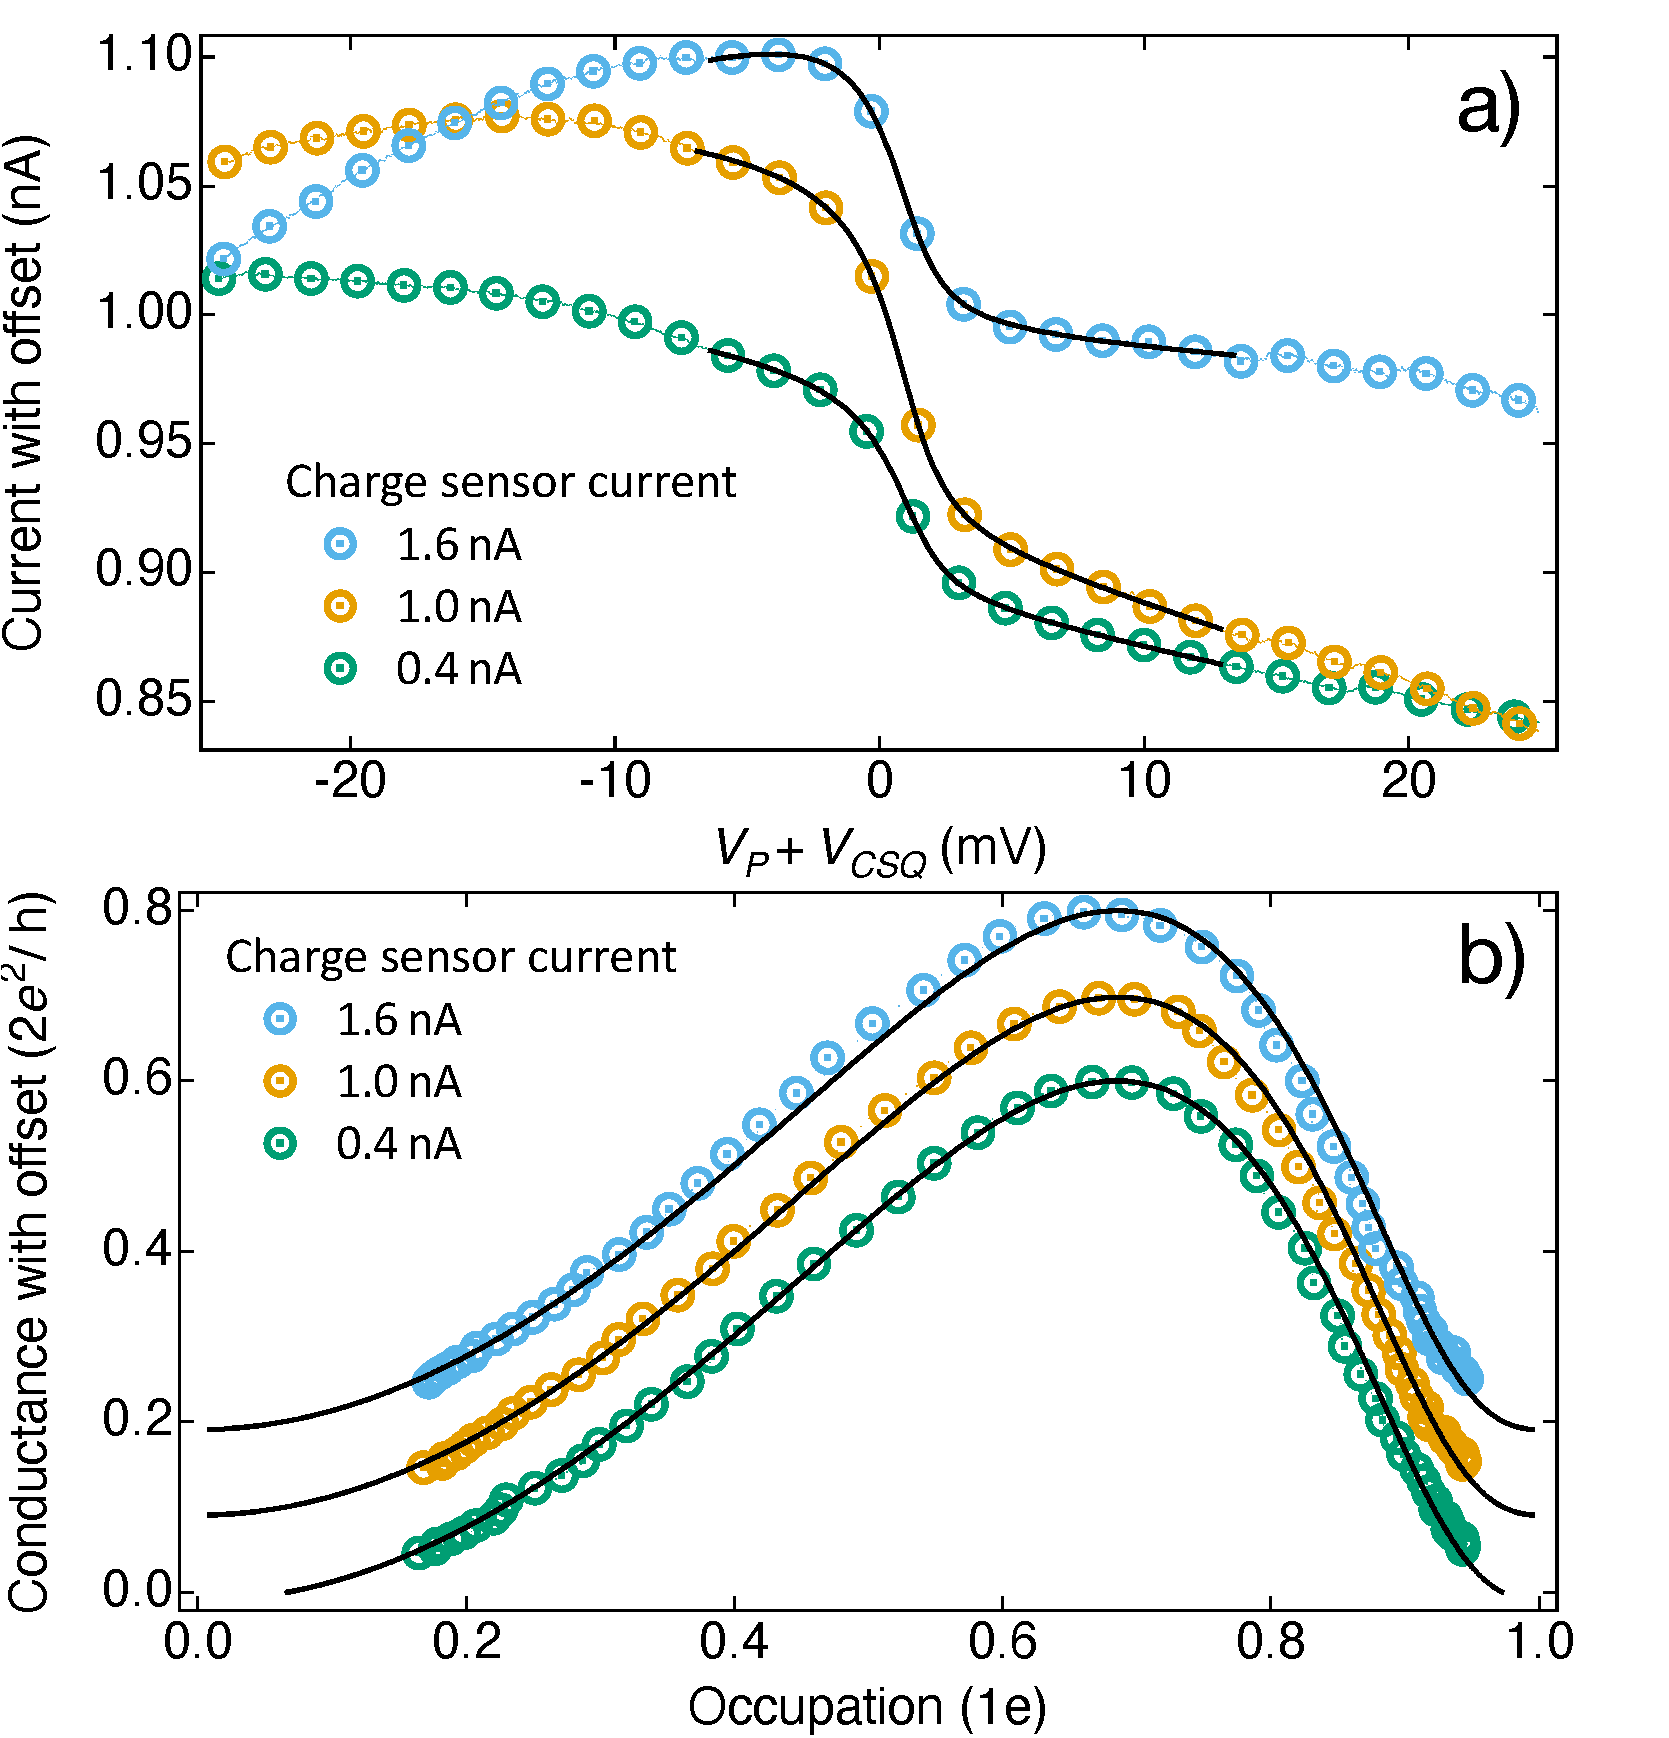
\includegraphics[width=0.85\textwidth]{figures/ch3/figure17.pdf}
 \caption[Conductance versus Occupation : Varying Charge Sensor Current]{\label{fig:ch3/cond_occ_QPC_vs_ct} 
 % For some options that work with pdf\LaTeX, please see this discussion:
 % \url{http://tex.stackexchange.com/questions/11839}. 
 (\textbf{a}) Charge transitions are measured with high (blue) and low (green) current through the charge sensor. For clarity, the transitions are offset in the current. The x-axis uses the same virtual gate for each charge transition. The slopes on either side of the charge transitions vary with the current through the charge sensor, suggesting the best virtual gate also changes. (\textbf{b}) Conductance versus occupation ($\mathrm{\Gamma/k_BT=21}$) at different current setpoints through the charge sensor. The traces are offset for clarity. Each trace is taken at \qty{20}{mK}. The coupling strength $\mathrm{\Gamma/k_BT}$ was determined from a global fit to conductance at multiple temperatures. The NRG (grey) conductance versus occupation, corresponding to the determined $\mathrm{\Gamma/k_BT}$, is plotted on top of the data. Good agreement is found at each current setpoint.}
 \end{center}
\end{figure}


Figure~\ref{fig:ch3/cond_occ_QPC_vs_ct}\textbf{a} shows charge transitions taken at \qty{20}{mK} for three different current setpoints through the charge sensor. For clarity, each charge transition has been offset in the current. The shape of the charge transition clearly depends on the current through the charge sensor. The unoccupied (left) side of the high current (blue) charge transition slopes down, whilst the low current (green) charge transition slopes upwards. This suggests that the optimal virtual gate to keep the charge sensor current constant also changes. At each current setpoint, conductance was simultaneously measured at a range of temperatures. A global fit to the conductance was used to determine $\mathrm{\Gamma/k_BT}$ and lever arm. Each charge transition was converted into an occupation, and the conductance versus occupation is plotted with a comparison to NRG (Fig.~\ref{fig:ch3/cond_occ_QPC_vs_ct}\textbf{b}). For clarity, the conductance versus occupation traces have each been offset by \qty{0.1}{2e^2/h}. Excellent agreement between data and NRG is found at each current setpoint. 


% \afterpage{\clearpage}
\section{Kondo Effect with Varying Coupling Symmetry}

All previous conductance data shown in this thesis was taken with symmetric coupling ($\mathrm{\Gamma_R = \Gamma_L}$). Previous measurements of the Kondo effect also tune the quantum dot to be symmetrically coupled with the source and drain leads. However, some experimental studies have investigated the Kondo effect with asymmetric coupling ($\mathrm{\Gamma_R \neq \Gamma_L}$)~\cite{kondo_asymmetric}. It was found that the characteristic zero bias peak between Coulomb peaks shifted to a nonzero bias. However, this effect would require a strong energy dependence of the tunnel barriers (i.e., $\mathrm{\Gamma = \Gamma(E)}$) in a NRG calculation, which is not assumed in our current NRG calculations.
Hence, a measurement of conductance with nonzero bias cannot be currently compared to NRG. 
Although we may not quantitatively corroborate these previous findings, exploring coupling symmetry is interesting as it effectively tests how the Kondo enhancement varies when a quantum dot is coupled to two leads (symmetric case) versus a single lead (asymmetric case). In practice, the limit of a single lead regime cannot be reached, as conductance will not be measured through the quantum dot.


% \afterpage{\clearpage}
\subsection{Symmetric to Asymmetric}


\begin{figure}[!hbt]
 \begin{center}
%% includegraphics: comment the following if not using the graphicx package
 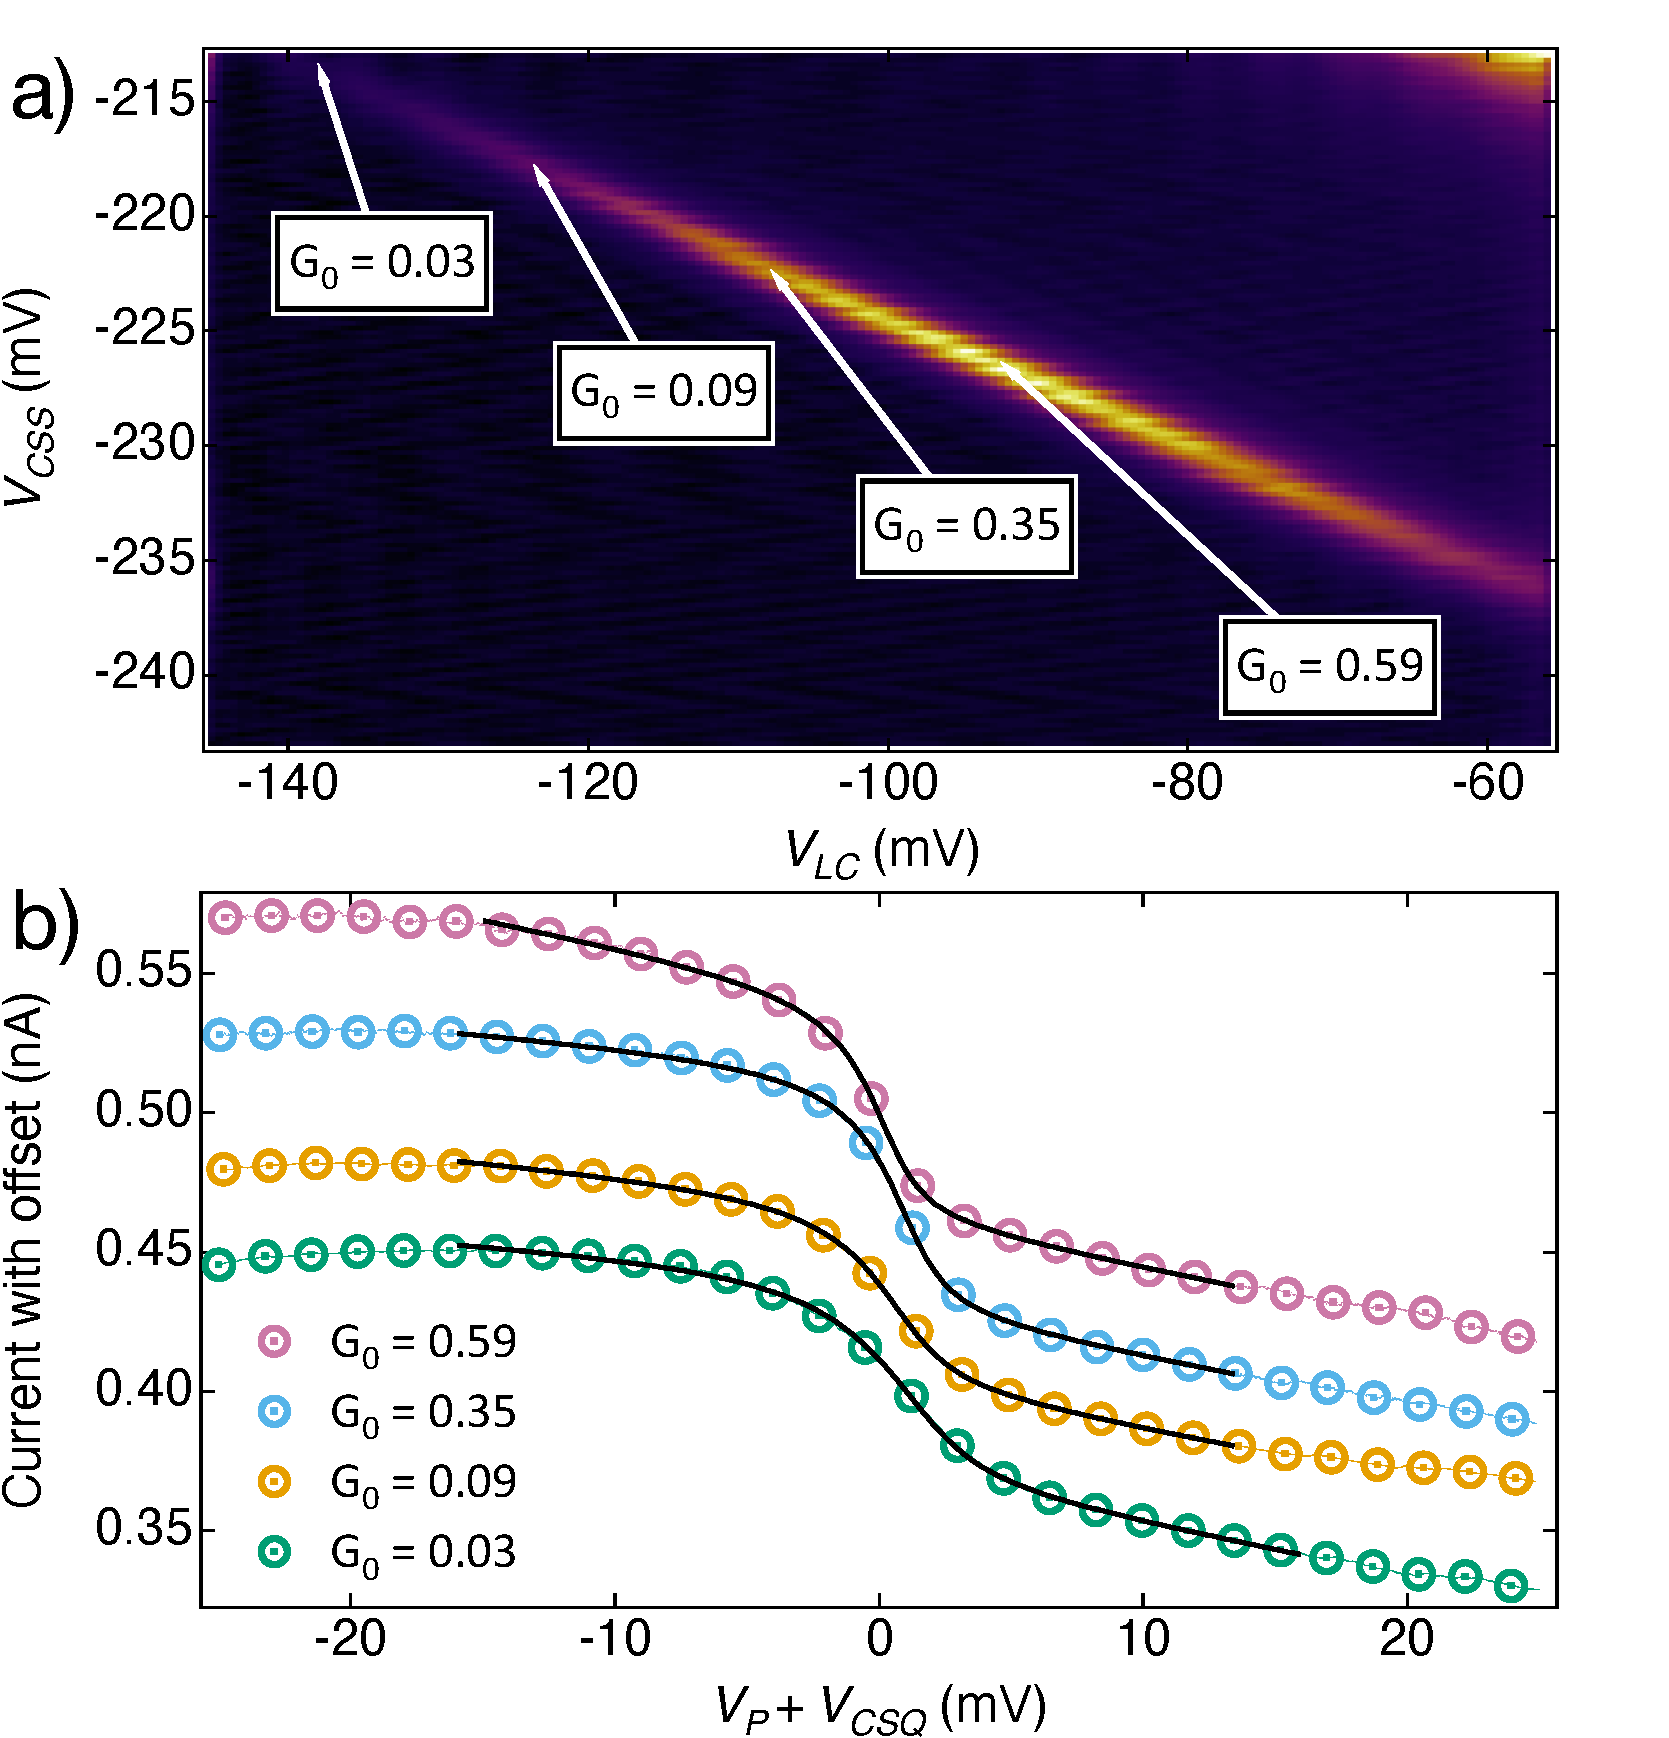
\includegraphics[width=0.85\textwidth]{figures/ch3/figure18.pdf}
 \caption[Symmetric to Asymmetric Coupling]{\label{fig:ch3/symmetry_picking} 
 % For some options that work with pdf\LaTeX, please see this discussion:
 % \url{http://tex.stackexchange.com/questions/11839}. 
 (\textbf{a}) 2D scan of conductance through the quantum dot varying the two coupling gates V\textsubscript{CSS}, and V\textsubscript{LC}. In the top left, the dot is more coupled to the right lead than the left as V\textsubscript{LC} is made more negative. In the middle of the scan (where the conductance is maximum), the coupling is symmetric $\mathrm{\Gamma_R} = \mathrm{\Gamma_L}$ (\textbf{b}) Charge transitions measured with different ratios of coupling between the two leads in the dot. $\mathrm{G_0} = 0.59$ is symmetric coupling (pink), $\mathrm{G_0} = 0.03$ is asymmetric coupling (green). For clarity, the transitions are offset in the current. But have been measured with roughly the same current setpoint through the charge sensor ($\sim\qty{0.4}{nA}$). The x-axis uses the same virtual gate for each charge transition. 
 % The charge transitions become more strongly coupled as asymmetric increases (pink-green)
 }
 \end{center}
\end{figure}


The width of a strongly coupled Coulomb peak is controlled by $\Gamma$. Where $\Gamma$ is the sum of the individual tunnelling rates, $\Gamma=\mathrm{\Gamma_L} + \mathrm{\Gamma_R}$. 
The conductance amplitude in both the weakly (Eq.~\ref{eq:cond_amp}) and strongly (Eq.~\ref{eq:cond_amp_strong}) coupled regimes depend on $\Gamma$. Hence, the conductance amplitude can be used as a marker of how asymmetrically coupled the quantum dot is to the leads. 


To vary the coupling symmetry in a quantum dot, a 2D scan measuring the conductance with gates that control a separate coupling on each axis is used. In Fig.~\ref{fig:ch3/symmetry_picking}\textbf{a}, V\textsubscript{CSS} (y-axis) mainly controls $\mathrm{\Gamma_R}$, and V\textsubscript{LC} (x-axis) mainly controls $\mathrm{\Gamma_L}$. Four points are picked from symmetric coupling (middle of scan) to asymmetric coupling (top left of scan), where the dot becomes more strongly coupled to the right lead. 
% The ratio $\mathrm{\Gamma_L}/\mathrm{\Gamma_R}$ was only calculated after the conductance global fit to NRG, which determined $\Gamma$. 




Charge transitions were simultaneously measured so that conductance versus occupation could be compared with the corresponding NRG. 
Charge transitions for each coupling setpoint were measured with $\sim\qty{0.4}{nA}$ through the charge sensor (Fig.~\ref{fig:ch3/symmetry_picking}\textbf{b}). 
Each charge transition did not have charge jumps near the transition and was deemed a reliable measure of the occupation. Interestingly, the asymmetrically coupled transition (green) is more broadened than the symmetrically coupled transition (pink). $\mathrm{\Gamma/k_BT}$ determined from the global fit to conductance varied from 20.5 for symmetric coupling to 26.0 for asymmetric coupling. However, a global fit to the charge transitions finds 19.6 for symmetric coupling and 45.0 for asymmetric coupling (Table~\ref{tab:sym_coupling_gf}). 
% \newcolumntype{P}[1]{>{\centering\arraybackslash}p{#1}}

\begin{table}[!hbt] 
\centering
\begin{tabular}{|c|c|c|}
% \begin{tabular}{|c{2.0cm}|c{4.0cm}|c{4.0cm}|}
\hline
\multicolumn{1}{|c|}{} & \multicolumn{2}{c|}{$\mathrm{\Gamma/k_BT}$ from Global Fit}\\
\hline
 $\mathrm{G_0}\,(\qty{}{2e^2/h})$ & Conductance Fit & Charge Transition Fit \\
\hline
0.59 & 20.5 & 19.6 \\
0.35 & 22.0 & 21.6 \\
0.09 & 24.4 & 30.9\\
0.03 & 26.0 & 45.0\\
\hline
\end{tabular}
 \caption[$\mathrm{\Gamma/k_BT}$ From Conductance and Charge Transition Global Fits]{\label{tab:sym_coupling_gf} $\mathrm{\Gamma/k_BT}$ determined from a global fit to conductance and separately a global fit to charge transitions at different ratios of coupling symmetry. At symmetric coupling ($\mathrm{G_0}=0.59$), the determined $\mathrm{\Gamma/k_BT}$ from conductance and charge transitions are similar. However, at asymmetric coupling ($\mathrm{G_0}=0.03$), the $\mathrm{\Gamma/k_BT}$ from a global fit to charge transitions is much greater than from a global fit to conductance.}
\end{table}


% \afterpage{\clearpage}
\subsection{Conductance versus Occupation}



\begin{figure}[!bht]
 \begin{center}
%% includegraphics: comment the following if not using the graphicx package
 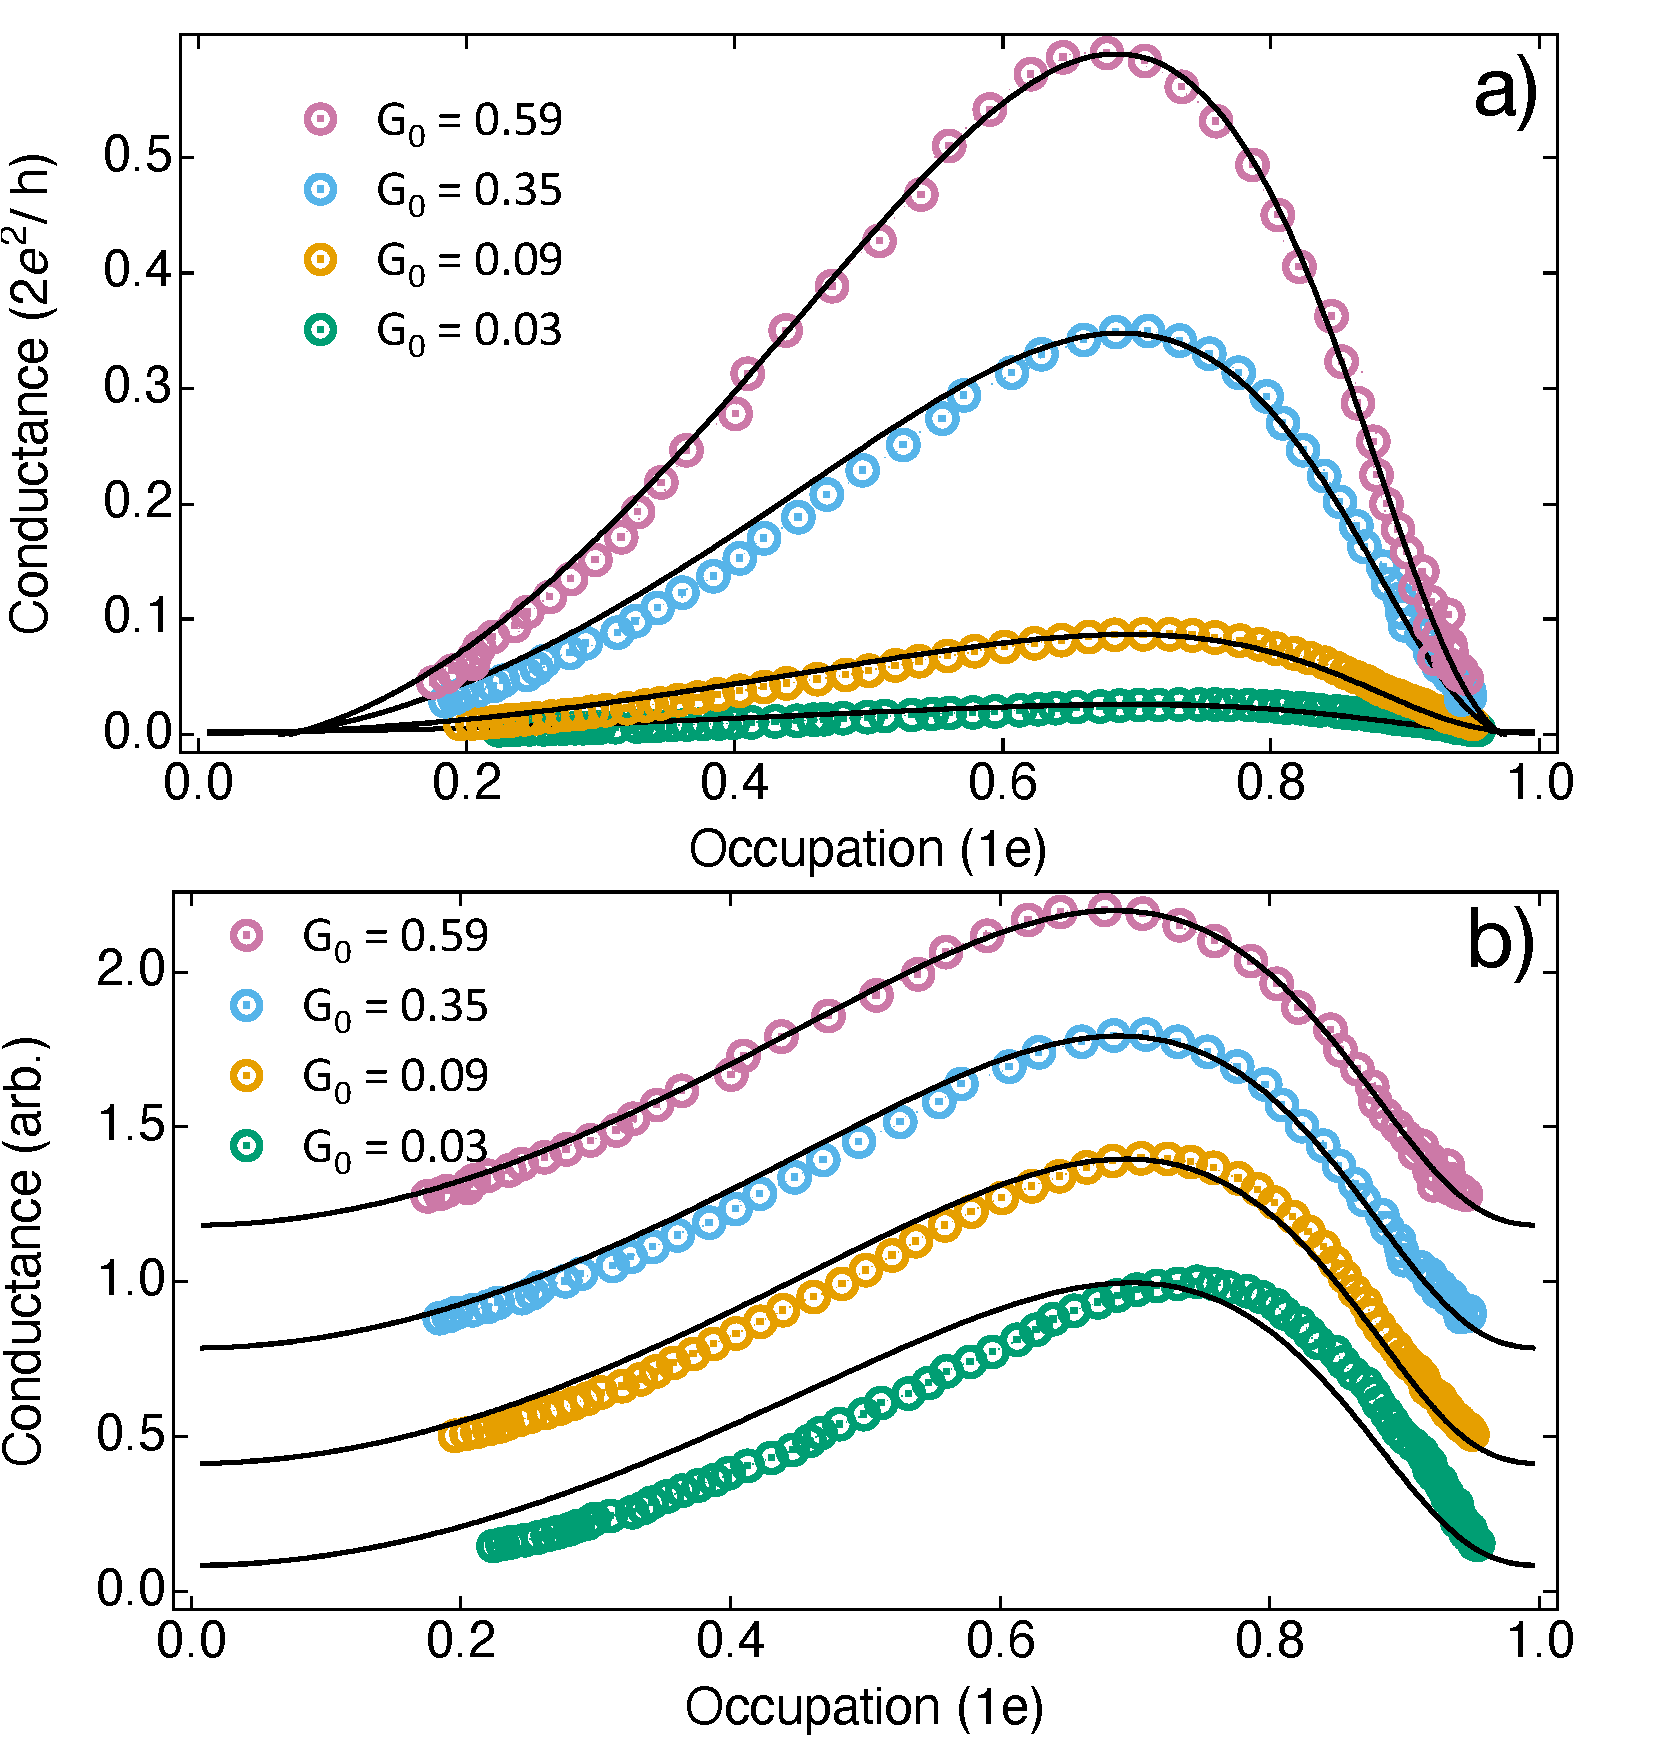
\includegraphics[width=0.85\textwidth]{figures/ch3/figure19.pdf}
 \caption[Conductance versus Occupation : Varying coupling symmetry]{\label{fig:ch3/cond_occ_assymetry} 
 % For some options that work with pdf\LaTeX, please see this discussion:
 % \url{http://tex.stackexchange.com/questions/11839}. 
 (\textbf{a}) Conductance versus occupation ($\mathrm{\Gamma/k_BT=21}$) with different ratios of coupling symmetry between the two leads of the dot. As the asymmetry is increased, the conductance decreases.
 (\textbf{b}) Same data as in (\textbf{a}), except the traces are offset and scaled for clarity. Symmetric coupling agrees well with NRG calculations. However, the asymmetrically coupled data is shifted to the right of the predicted NRG. This suggests that $\mathrm{\Gamma/k_BT}$ extracted from the global fit to conductance is lower than expected.}
 \end{center}
\end{figure}


Figure~\ref{fig:ch3/cond_occ_assymetry}\textbf{a} shows conductance versus occupation taken at \qty{20}{mK} at the four different ratios of coupling symmetry found in Fig.~\ref{fig:ch3/symmetry_picking}\textbf{a}. There is good agreement with NRG in the symmetric coupling (pink). However, as the coupling becomes more asymmetric, the conductance amplitude decreases (Eq.~\ref{eq:cond_amp_strong}), and agreement with NRG is difficult to determine. Hence, for clarity, Fig.~\ref{fig:ch3/cond_occ_assymetry}\textbf{b} shows the same data with an added scaled and offset. The corresponding NRG was also scaled and offset the same as the data. A disagreement between asymmetric coupling (green) data and NRG becomes much clearer. When asymmetrically coupled, the conductance maximum of the data is shifted to the right of the NRG. This suggests the $\mathrm{\Gamma/k_BT}$ determined from the global fit to conductance is lower than expected. 



This discrepancy with NRG is surprising as conversations with our theorist collaborators suggest that NRG only depends on the overall $\Gamma$, and not the ratio between $\Gamma_\mathrm{L}$ and $\Gamma_\mathrm{R}$.
Perhaps some mechanism could be altering the shape or location of the conductance. 
Previous experiments have used a charge sensor as a noise source to de-phase the Kondo singlet~\cite{kondo_controlled_dephasing}. In these studies, the bias across the charge sensor was \qty{1200}{\micro V}, twelve times the bias that is used for the charge sensor in this thesis (\qty{100}{\micro V}) and the suppression of the measured conductance was $\sim6\%$. 
A more recent theoretical study found that for weak coupling between the charge sensor and quantum dot, the spectral weight of the Kondo resonance is reduced, leading to a suppression of the conductance. However, the width of the resonance is not affected, suggesting the absence of dephasing~\cite{peculiar_dephasing_of_kondo}. Although this de-phasing mechanism could result in the conductance maximum being shifted to a lower occupation, it would not explain a shift to a higher occupation or the dependence on symmetric coupling.


Instead of a change in the shape or location of the conductance, it is possible the charge transition behaves differently between coupling symmetries. 
Numerous studies have investigated the tunnelling rates onto and off the quantum dot~\cite{MacLean2007,Ihn2009,Kng2012}, with differing barrier symmetries~\cite{Rogge2005,Gustavsson2006}. However, these studies required the source-drain bias to be larger than the temperature broadening, so the results cannot be extrapolated to our regime of zero bias. 

An early study on the shape of the charge transition with symmetric coupling found that in the absence of a magnetic field, charge transitions are unaffected by the onset of Kondo correlations~\cite{Sprinzak2002}. It was argued that the conductance enhancement between Coulomb peaks results from a larger number of electrons traversing the quantum dot, each dwelling there for a shorter time. However, coupling symmetry was not explored in this experiment. 


 The most promising insight comes from very recent theoretical studies of the differential conductance through a quantum dot and its dependence on asymmetry in the tunnel barriers and source-drain bias~\cite{Tsutsumi2021,kondo_nrg_asymmetric}. 
 It was found that higher-order corrections to the differential conductance include non-linear terms that depend strongly on the tunnelling and bias asymmetries. As an example, for $\Gamma_\mathrm{L}>\Gamma_\mathrm{R}$, the number of electrons entering the quantum dot from the left side becomes larger than the number of electrons leaving the right side. Therefore, the number of electrons in the dot increases and the repulsive interaction increases $\tilde{\epsilon}_0$. In contrast, $\tilde{\epsilon}_0$ would decrease for $\Gamma_\mathrm{L}<\Gamma_\mathrm{R}$. This modification to $\tilde{\epsilon}_0$ can result in increased or decreased conductance. 

It should be noted that the exploration of symmetric coupling in this thesis only came from two overnight measurements in a single cooldown and a second cooldown is required to verify the findings. Additionally, a subsequent cooldown would allow for a more focused exploration of tunnel coupling and bias symmetry. 
 




% \clearpage
% \section{Discussion}



